\documentclass[margin=3mm]{standalone}
\usepackage{tikz}
\usetikzlibrary{shapes, arrows}

\tikzstyle{startstop} = [rectangle, rounded corners, minimum width=2cm, minimum height=1cm, text centered, draw=black, text=white, fill=black!80]
\tikzstyle{statement} = [rectangle, minimum width=4cm, minimum height=1cm, text centered, draw=black, fill=blue!20]
\tikzstyle{decision} = [rectangle, minimum height=1cm, text centered, draw=black, fill=yellow!30]
\tikzstyle{edge} = [thick, ->, >=stealth]

\begin{document}
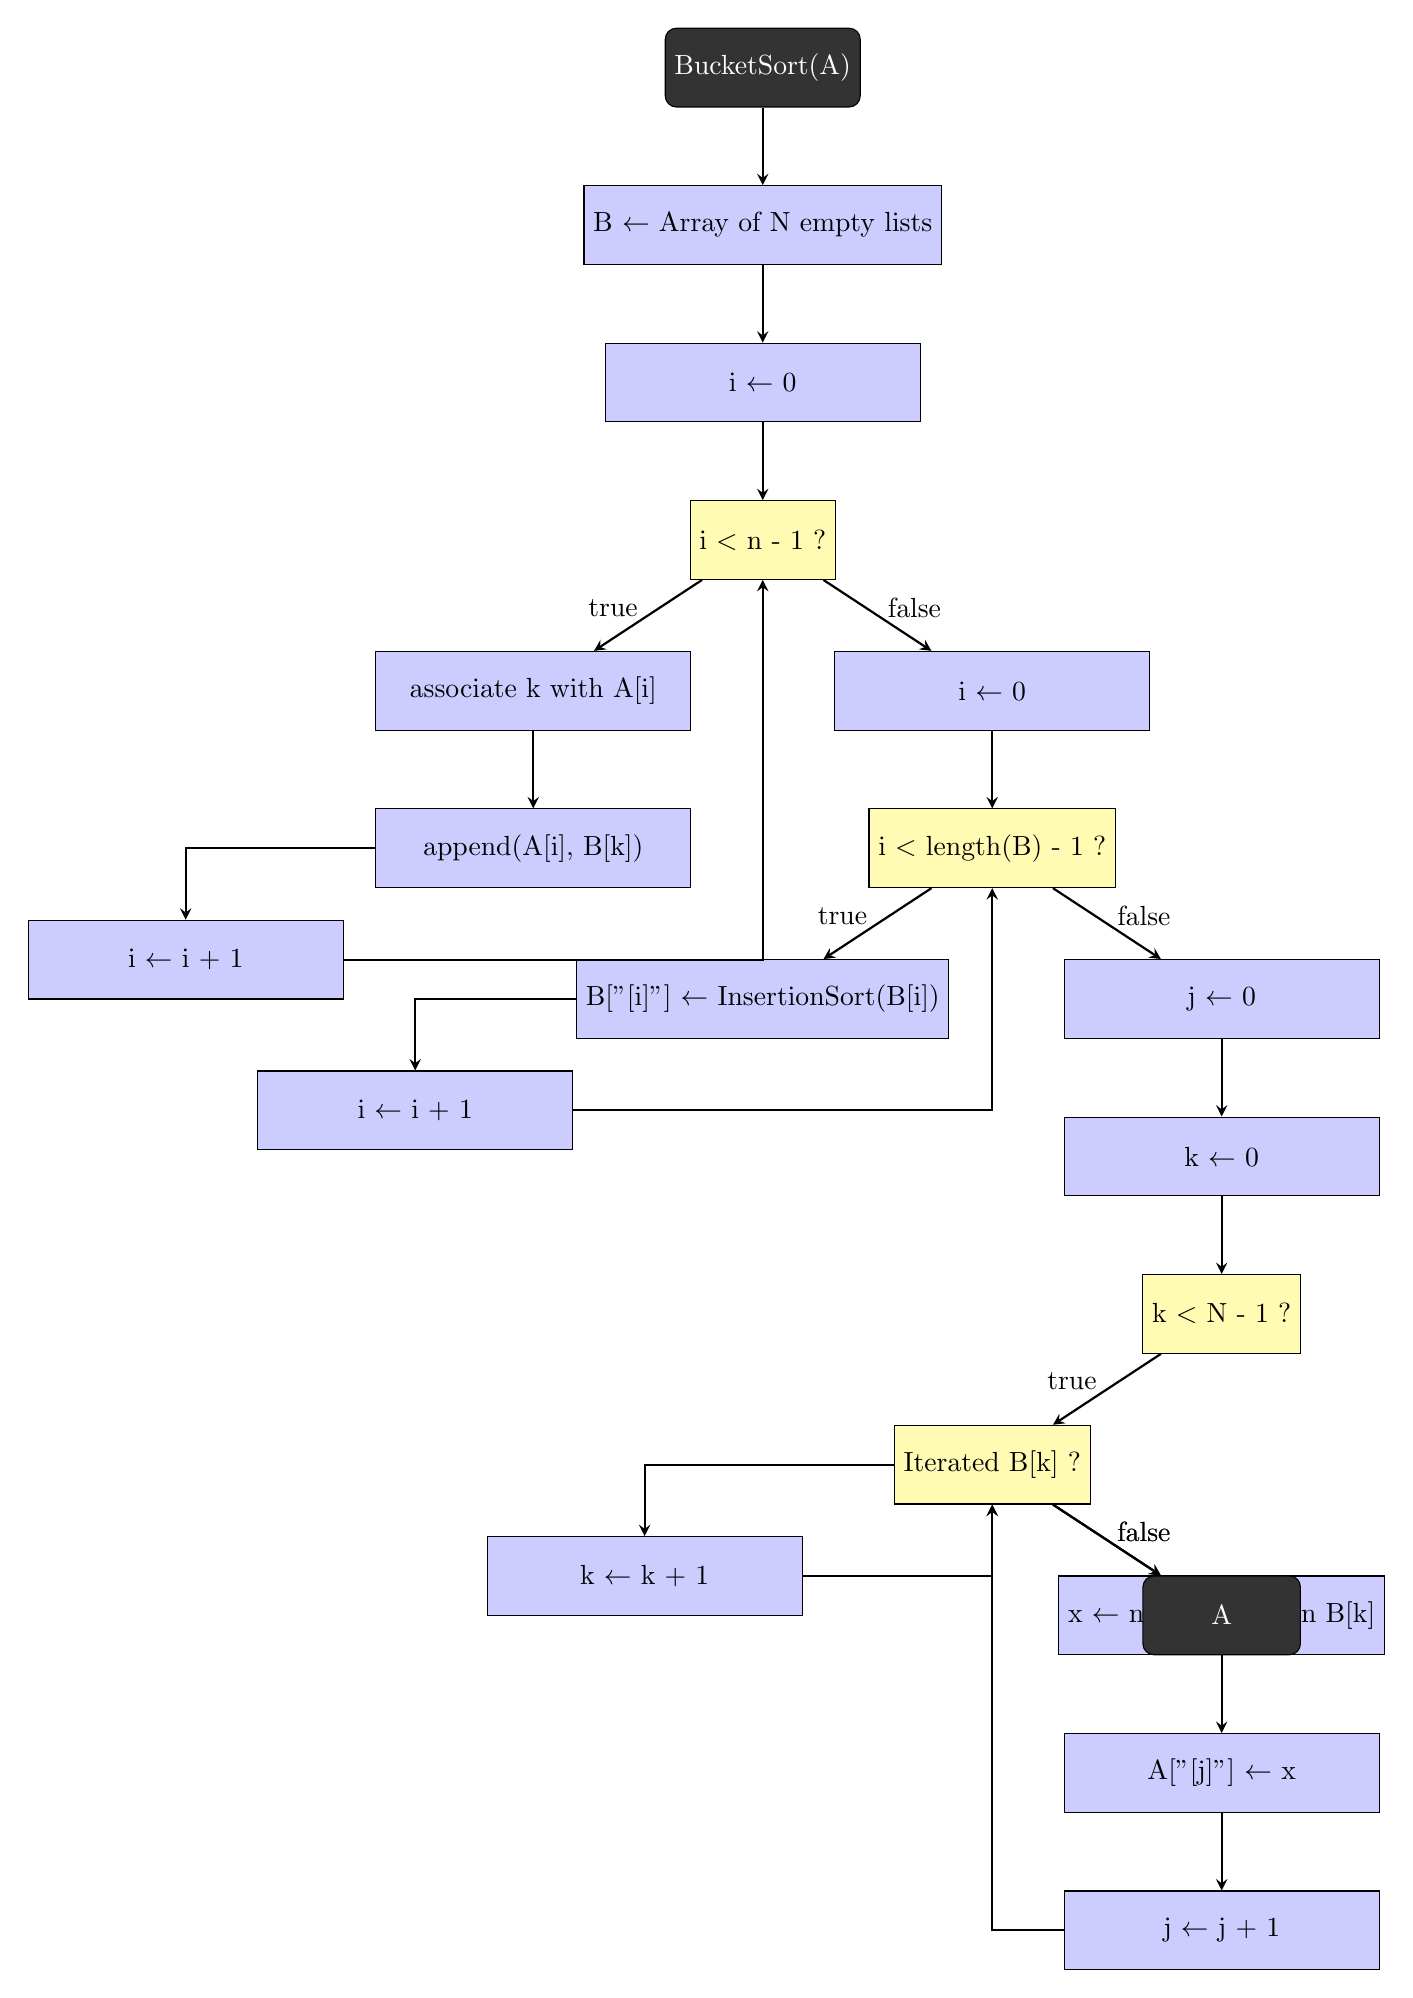
\begin{tikzpicture}[node distance=2cm]

\node (0) [startstop] {BucketSort(A)};
\node (1) [statement, below of=0] {B $\gets$ Array of N empty lists};
\node (2) [statement, below of=1] {i $\gets$ 0};
\node (3) [decision, below of=2] {i $<$ n - 1 ?};
\node (4) [statement, yshift=-0.5cm, xshift=-1.5cm, below left of=3] {associate k with A[i]};
\node (5) [statement, below of=4] {append(A[i], B[k])};
\node (6) [statement, xshift=-3cm, below left of=5] {i $\gets$ i + 1};
\node (7) [statement, yshift=-0.5cm, xshift=1.5cm, below right of=3] {i $\gets$ 0};
\node (8) [decision, below of=7] {i $<$ length(B) - 1 ?};
\node (9) [statement, yshift=-0.5cm, xshift=-1.5cm, below left of=8] {B["[i]"] $\gets$ InsertionSort(B[i])};
\node (10) [statement, xshift=-3cm, below left of=9] {i $\gets$ i + 1};
\node (11) [statement, yshift=-0.5cm, xshift=1.5cm, below right of=8] {j $\gets$ 0};
\node (12) [statement, below of=11] {k $\gets$ 0};
\node (13) [decision, below of=12] {k $<$ N - 1 ?};
\node (14) [decision, yshift=-0.5cm, xshift=-1.5cm, below left of=13] {Iterated B[k] ?};
\node (15) [statement, yshift=-0.5cm, xshift=1.5cm, below right of=14] {x $\gets$ next element in B[k]};
\node (16) [statement, below of=15] {A["[j]"] $\gets$ x};
\node (17) [statement, below of=16] {j $\gets$ j + 1};
\node (18) [statement, xshift=-3cm, below left of=14] {k $\gets$ k + 1};
\node (19) [startstop, yshift=-0.5cm, xshift=1.5cm, below right of=14] {A};

\draw [edge] (0) -- (1);
\draw [edge] (1) -- (2);
\draw [edge] (2) -- (3);
\draw [edge] (3) -- node[anchor=west, yshift=0.1cm]{false} (7);
\draw [edge] (3) -- node[anchor=east, yshift=0.1cm]{true} (4);
\draw [edge] (4) -- (5);
\draw [edge] (5) -| (6);
\draw [edge] (6) -| (3);
\draw [edge] (7) -- (8);
\draw [edge] (8) -- node[anchor=west, yshift=0.1cm]{false} (11);
\draw [edge] (8) -- node[anchor=east, yshift=0.1cm]{true} (9);
\draw [edge] (9) -| (10);
\draw [edge] (10) -| (8);
\draw [edge] (11) -- (12);
\draw [edge] (12) -- (13);
\draw [edge] (13) -- node[anchor=east, yshift=0.1cm]{true} (14);
\draw [edge] (14) -- node[anchor=west, yshift=0.1cm]{false} (19);
\draw [edge] (14) -| (18);
\draw [edge] (14) -- node[anchor=west, yshift=0.1cm]{false} (15);
\draw [edge] (15) -- (16);
\draw [edge] (16) -- (17);
\draw [edge] (17) -| (14);
\draw [edge] (18) -| (14);

\end{tikzpicture}
\end{document}